% This work is licensed under the Creative Commons
% Attribution-NonCommercial 3.0 Unported License.  To view a copy of
% this license, visit http://creativecommons.org/licenses/by-nc/3.0/.

\section{Aufbau und Durchführung}

\subsection{Aufbau einer Apparatur zur Bestimmung der Suszeptibilität}
\label{sec:aufbau-apparatur}

Die Apparatur besteht im wesentlichen aus vier Teilen: Einem
Funktionengenerator als Signalgeber, einer Brückenschaltung, einem
Verstärker und einem Meßgerät.  Der Signalgeber speist die
Brückenschaltung mit einem Sinussignal, ein Verstärker leitet das Signal
verstärkt an das Meßgerät weiter.  Ein Schema der Versuchsanordnung ist
in \cref{fig:schema-aufbau} skizziert.  Das Prinzip, nach dem die
Suszeptibilität bestimmt wird, basiert auf einer Induktivitätsmessung
einer Spule, in welche die zu messende Probe eingeführt wird.  Der
Verstärker ist notwendig, da die auftretenden Spannungen sehr gering
sind und von Störspannungen, die in dieser Größenordnung immer
auftreten, überlagert sind.  Aus diesem Grunde ist zusätzlich ein Filter
in den Verstärker integriert, da das zu messende Signal monofrequent,
die Störsignale aber ein Frequenz-Spektrum haben können, das viele
verschiedene Frequenzen enthält.

\begin{figure}
  \centering
  \includegraphics[width=\textwidth]{aufbau}
  \caption{Der Aufbau der Versuchsanordnung.  Der Sinusgenerator liefert
    die Speisespannung für die Brücke in Form einer monofrequenten
    Sinuswelle.  Die Brücke dient zum Messen der Induktivität der Spule,
    in die die Probe eingelegt wird.  Der Selektivverstärker filtert
    Störungen heraus und verstärkt das Signal, das an der Brücke anliegt
    und das Meßgerät mißt die Spannung.}
  \label{fig:schema-aufbau}
\end{figure}

\subsubsection{Beschreibung der Brückenschaltung}

Die Brücke zur Induktivitätsmessung ist in \cref{fig:bruecke}
skizziert.  In das Innere der Spule, die mit $L_\text{M}$ bezeichnet ist,
kann die zu untersuchende Probe eingeführt werden.  Durch das Einführen
einer Probe mit Querschnitt~$Q$ und magnetischer Suszeptibilität~$\chi$
in eine Spule der Länge~$l$ und Windungszahl~$n$ ist der Unterschied
zwischen der Induktivität~$L_\text{M}$ und $L$ um
\begin{equation}
  \Delta L = \mu_0 \chi Q \frac{n^2}{l}.
\end{equation}
Der Zusammenhang zwischen Brückenspannung~$U_\text{Br}$ und magnetischer
Suszeptibilität~$\chi$ ergibt sich aus den Abgleichbedingungen für die
Brücke.  Es gilt:
\begin{equation}
  \label{eq:chi-spannungen}
  \chi = \frac{U_\text{Br}}{U_\text{Sp}} \frac{4 l}{\omega \mu_0 n^2 Q}
  \sqrt{R^2 + \omega^2 \left(\mu_0 \frac{n^2}{l} F\right)^2},
\end{equation}
wobei hier $F$ die Querschnittsfläche der Spule und $U_\text{Sp}$ die
Speisespannung bezeichnet.  Wird nun in die ohne eingelegte Probe
abgeglichene Brücke die Probe eingeführt, dann ergibt sich ebenfalls aus
den Abgleichbedingungen der Brücke, daß der Widerstand~$R_3$ sich um
\begin{equation}
  \label{eq:delta-r}
  \Delta R = \chi \frac{R_3 Q}{2 F}.
\end{equation}

\begin{figure}
  \centering
  \includegraphics[height=5cm]{bruecke}
  \caption{Schaltskizze der verwendeten Meßbrücke.  Sie dient dazu die
    Induktivität zu messen.  In die Spule~$L_\text{M}$ wird die Probe
    eingelegt. Der Widerstände~$R_3$ und $R_4$ sind als
    Präzisionspotentiometer ausgeführt.  Die Abbildung ist aus
    \textcite{v606} entnommen.}
  \label{fig:bruecke}
\end{figure}

\subsubsection{Unterdrückung von Störspannungen}

Wie bereits erwähnt treten an den Ausgangsklemmen der Brückenschaltung
Störspannungen auf.  Da die zu messende Brückenspannung vermutlich
völlig von den Störungen verdeckt wird, muß ein Weg gefunden werden,
diese herauszufiltern.  Man wählt dazu als Speisespannung ein
Sinussignal und verwendet einen Selektivverstärker, der nur Spannungen
im Bereich der Frequenz dieses Signals herum passieren läßt.  Da die
Störspannungen viele verschiedene Frequenzen enthalten, kann ein
Großteil der Störungen herausgefiltert werden.  Die Güte
\begin{equation}
  \label{eq:guete}
  Q = \frac{\nu_0}{\nu_+ - \nu_-}
\end{equation}
ist ein Maß für die Schärfe des Bereichs, in dem die ungewollten
Frequenzen abgeschnitten werden.

\subsection{Messung der Güte des Selektivverstärkers}

Zu allererst wird eine Güte-Messung des verwendeten Selektivverstärkers
durchgeführt.  Dazu wird ein Sinussignal vom Funktionengenerator in den
Eingang des Verstärkers gegeben und am Ausgang von einem Meßgerät wieder
abgenommen.  Jetzt wird die Frequenz des Sinussignals verändert und so
eine Meßreihe Spannung gegen Frequenz durchgeführt.  Ziel ist es,
herauszufinden, wie gut die Filtereigenschaften des Selektivverstärkers
sind.  Die Meßwerte werden um den Bereich der Resonanzspitze dichter
gewählt, um eine bessere Auflösung gewährleisten zu können.

\subsection{Messung der Suszeptibilität der Proben}

Wie bereits in \cref{sec:aufbau-apparatur} angerissen, wird die
Suszeptibilität der Proben über eine Induktivitätsmessung realisiert.
Die Induktivitäten werden mithilfe einer Brückenschaltung und der
Nullmethode bestimmt, um eine gute Genauigkeit zu erreichen.  Da die
auftretenden Signale allerdings in der Größenordnung der Störungen
liegt, ist ein sogenannter Selektivverstärker notwendig, der das Signal
verstärkt und nur eine Frequenz durchläßt.

Es gibt zwei Möglichkeiten, mit der oben beschriebenen Apparatur die
Suszeptibilität zu bestimmen.  Wird bei ausgeglichener Brücke,
d.\,h. die Brückenspannung verschwindet, die Probe in die Spule
geschoben, so läßt sich aus der Änderung der Brückenspannung die
Änderung der Induktivität berechnen.  Die zweite Möglichkeit ist nun,
die Brücke mit eingelegter Probe auszugleichen und daraus die Änderung
der Induktivität abzulesen.  Hier werden beide Möglichkeiten
nacheinander ausgeführt, damit je zwei Meßwerte pro Messung erhalten
werden.

\subsection{Theoretische Vorhersage für die Suszeptibilitäten}

Am Ende sollen die experimentell bestimmten Werte mit der theoretischen
Vorhersage verglichen werden, um beurteilen zu können, wie gut das
quantentheoretische Modell den Paramagnetismus beschreibt.  Dazu muß
zunächst die Elektronenkonfiguration der 4f-Elektronen für die drei
Verbindungen Dy$_2$O$_3$, Gd$_2$O$_3$ und Nd$_2$O$_3$ bestimmt werden.
Hierfür werden die \name{Hund}schen Regeln verwendet.  Beispielhaft wird
die Berechnung von Dysprosium(III)-oxid durchgeführt.  Die beiden
Dysprosium-Atome haben die Elektronenkonfiguration [Xe]4f$^{10}$6s$^2$
und müssen jeweils drei Elektronen für die Bindung abtreten, daher
bleiben auf der 4f-Schale noch 9 Elektronen über.  Die Schale hat
insgesamt Platz für 14 Elektronen, 7 mit Spin-Up und 7 mit Spin-Down.
Nach der ersten \name{Hund}schen Regel ergibt sich, daß die 7 Plätze mit
Spin-Up voll besetzt und die übrigen 2 Elektronen Plätze mit Spin-Down
besetzen. Daher ist $S = 5/2$.  Nach der zweiten Regel ergeben besetzen
die zwei Spin-Down die Plätze der beiden höchsten magnetischen
Quantenzahlen 3 und 2.  Es gilt daher $L = 5$ und aus der dritten Regel,
da die Schale mehr als halb besetzt ist, folgt für die
Gesamtdrehimpulsquantenzahl $J = 15/2$.  Analog wird für die übrigen
vorgegangen.  Die Ergebnisse sind in \cref{tab:proben-daten} zu sehen.

\begin{table}
  \centering\footnotesize\sisetup{
    table-number-alignment = center,
    table-figures-integer = 1
    }
  \begin{tabular}{l
      S[table-figures-decimal=1]
      S[table-figures-decimal=0]
      S[table-figures-decimal=1]
      S[table-figures-decimal=2]
      S[table-figures-decimal=2,
        table-figures-integer=3]
      S[table-figures-decimal=4]
      S[table-figures-decimal=2]
      S[table-figures-decimal=4]}
    \toprule
    Verbindung & {$J$} & {$L$} & {$S$} & {$\rho/(\si{g/cm^3})$} &
    {$M/(\si{g/mol})$} & {$N/(10^{28} \si{m^{-3}})$} & {$g_J$} & {$\chi$} \\
    \midrule
    Dy$_2$O$_3$ [Xe]4f$^{10}$6s$^2$ &
    7.5 & 5 & 2.5 & 7.8  & 373 & 2.5186 & 1.33 & 0.0251\\
    Nd$_2$O$_3$ [Xe]4f$^4$6s$^2$ &
    4.5 & 6 & 1.5 & 7.34 & 336.48 & 2.6273 & 0.73 & 0.0030\\
    Gd$_2$O$_3$ [Xe]4f$^7$5d6s$^2$ &
    3.5 & 0 & 3.5 & 7.4  & 362.49 & 2.4588 & 2.00 & 0.0136\\
    \bottomrule
  \end{tabular}
  \caption{Die Quantenzahlen ergeben sich aus den \name{Hund}schen
    Regeln.  Die anderen Größen, die zur Berechnung der
    Suszeptibilität~$\chi$ benötigt werden, sind ebenfalls gelistet.  Da
    die Verbindung zwei Dy-Atome enthält gilt für die Teilchendichte $N
    = 2 \rho/M$, wobei $M$ die molare Masse der Probe bezeichnet.  Der
    \name{Landé}-Faktor, welcher sich aus den Quantenzahlen bestimmt,
    ist ebenfalls angegeben.}
  \label{tab:proben-daten}
\end{table}
